\documentclass{article}
\usepackage{CJKutf8}
\usepackage[utf8]{inputenc}
\usepackage{geometry}
\usepackage{fancyhdr}
\usepackage{array}
\usepackage{listings}
\usepackage{layouts}
\usepackage{graphics}
\usepackage{graphicx}
\usepackage{url}
% Note that you can only edit the content but not the page format
% Please modified below brackets with your team's information.
\def \teamno {10}
\def \teammembers {B09902005, B09902013, B09902096}
\def \bestranking {34 (on 20210625)}
\def \bestscore {76113.62}

\geometry{
    a4paper,
    total={7in, 9.5in},
    top=1.1in
}

\renewcommand{\footrulewidth}{0.4pt}
\fontfamily{charter}\selectfont
\pagenumbering{gobble}
\linespread{1.2}

\pagestyle{fancy}
\fancyhf{}
\rhead{Team No.\teamno}
\lhead{DSA Final Project Report}
\lfoot{Ranking: \bestranking \quad Score: \bestscore}
\rfoot{\teammembers}

% If you want to use Chinese, then you need to wrap the Chinese content with \begin{CJK}{UTF8}{bsmi} and \end{CJK}
% For example: \begin{CJK}{UTF8}{bsmi} 中文內容 \end{CJK}

\begin{document}

\section*{Data Structures \& Algorithms}

\textbf{Preprocessing:}

We hash the names (\verb|from| and \verb|to|) of mail to \verb|int| and we hash tokens to \verb|long long int|, and save them in our mail structure. By "observing" in our computer, we found a hash function for names without collision, which is 
\begin{verbatim}
name_hash(char name[])
    int r = 0, i = 0;
    while (name[i] != NIL)
        r = r * 128
        r = r + ASCII(name[i])
        r = r % 19815
        i = i + 1
    return r
\end{verbatim}
Since the value of ASCII is always less than $128$, and that $128$ is $2^7$, we use left shift (\verb|<<|) instead of multiplication and bitwise-OR instead of addition. It helps us to save some time.

As for the tokens, we cannot find a hash function with appropriate size of hash space and without collision yet. The least collision so far is $16$ out of $131078$ tokens at total. Our hash function for tokens is basically Rabin-Karp-like, similar to that for names, changing the multiplier, the modular base and the value each character represents.

Also, the hash space is so large that it takes too much time to initialize the space. Thus we use a set taught by Professor Lu which does not need to initialize the space. The basic thought is to have two array pointing at each other, an element exists in the set iff the position of the value points to the position of the index, and the position of index points to the position of value. To avoid they accidentally points to each other, we stores value of size such that if the index is greater than size, we know that it is not in the set. After hashing all the tokens, we sort the hash value in ascending order such that we can apply binary search on it.

As a comparison, we also use a data structure named trie to solve this problem. The concept of trie is to build a tree, which has letters on the edge, and every node represents a string which starts from root. In addition, we need to mark the node where a input string ends here so that we can recognize whether a string is from input or just a prefix. Below is a trie which stores strings \verb|abc|, \verb|abd|, \verb|adc|, \verb|bdc|, \verb|bda|, \verb|a|, \verb|bd|. The node where a input string ends at is marked with \verb|*|: (In order to make the graph easy to understand, we mark the string which the node represents on it. However, trie does not store the string.)

\begin{center}
    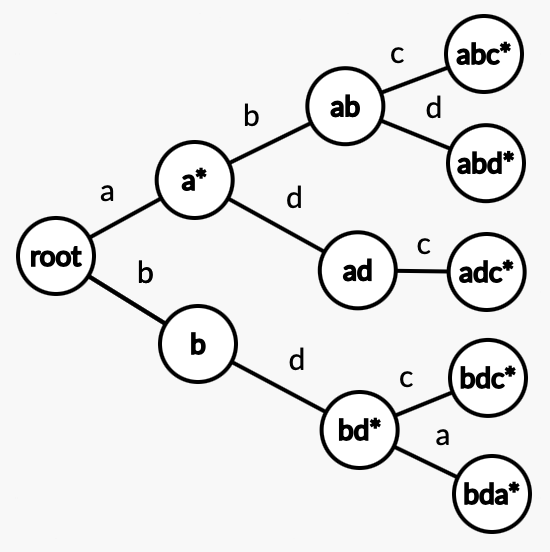
\includegraphics[width=0.35\textwidth]{pictures/trie.png}
\end{center}

Trie supports two operation:

\begin{enumerate}
    \item \verb|insert|: insert a given string \verb|s| into a trie.
    \item \verb|query|: query for whether a given string \verb|s| is in the trie.
\end{enumerate}

Both can be easily implemented by delete the first character of string and determine which children to go to recursively. The source code can be view at \url{https://github.com/b20896916/email-searcher/blob/main/trie.c}.

During preprocessing, in order to build the trie for every mail, we start from a empty node, and then insert string step by step.\\ \\
\textbf{Expression Match:}

We deal with the expression first. We convert the expression (\verb|char[]|) into a post-fix linked list (stack). (Like we did in the course about stack in the first half of the semester.)
This takes us $O(l_e)$ time and space to convert, where $l_e$ is the length of expression.

After completing the post-fix linked list, we can now use it to see which mails return true with this expression.

For each mail, all tokens in the linked list can be viewed as true or false, which means whether the mail contains this token.

(Since we use binary search to search for a hash value in a mail, we need $O(\log l_m)$ time to determine the existence of a token, where $l_m$ is the length of a mail. So totally, we spend $O(n l_e \log l_m)$ time on it, where $n$ is the number of mails.)(Note that $l_e = 2048$, $l_m = 100000$.)

Finally, we can calculate the result, which takes $O(l_e)$ time.

When using trie to solve this problem, we can do whatever similar to hash but uses the \verb|query| operation trie supports instead of binary search to check whether a token is in the mail. The complexity is similar to hash, but the step of check takes $O(l_t)$, where $l_t$ is the maximum length of tokens, instead of $O(\log l_e)$\\ \\
\textbf{Find Similar:}

Since we have created ascending arrays that stores hash values of all tokens of the mails, if we want to know the similarity of two mails, all we have to do is to find the number of hash values that appear in both of their arrays.

Since the array is ascending, we can traverse from small to large numbers in the two arrays and only spend $O(l_m)$ time, where $l_m$ is the length of a mail to find the number of hash values appearing in both arrays. Let this number be $x$, then similarity can be obtained by $x / (size_a + size_b - x)$, where $size_a$ and $size_b$ is the size of the two arrays.

If we calculate the similarity this way for all emails with the given email, and compare them all with threshold, then this query is done.\\ \\
\textbf{Group Analysis:}

The problem is to find the number of connected components, $n_g$, and the size of the largest one, $l_g$, where each name of a mail is a vertex and each mail is an edge. 

We use disjoint set as our data structure, and union by size and path compression as our techniques.

Every time we do \verb|makeset|, the number of connected components increases by $1$. On the other hand, every time we do \verb|union|, the number of connected components decreases by $1$. Also, we check if the new union set is the currently largest.

Thus, with the details above, once we saw a mail, we union the hash value of the names. Then we will have $n_g$ and $l_g$ after visiting the whole subset of mails.\\


\section*{Cost Estimations of Queries}

\textbf{Preprocessing:}

Since we hashed the mail into numbers, including names and tokens, and our hash function is Rabin-Karp-based, thus our complexity of hashing is $O(nl_m)$.

After that, sorting takes $O(n_t\log{n_t})$, where $n_t$ is the sum of number of tokens in every mail.

When we do it with trie, we need to insert every token to trie for each mail. It's trivial that inserting a string with length $k$ require $k$ operation to reach the node it belongs to, so the time complexity is linear to the sum of string length stored in trie. The space of a trie is also surely the sum string length stored in it, because the worst case is that there is no strings share the same node except root. As a result, preprocessing of a mail is $O(l_m)$ time complexity, $O(l_m)$ space complexity. Preprocessing of all the $n$ mails requires $O(nl_m)$ time complexity, $O(nl_m)$ space complexity.\\ \\
\textbf{Expression Match:}

Our implementation solves Expression Match in $O(n l_e \log l_m)$ time and $l_e$ space, where $l_e$ is the length of the expression, (at most $2048$), and $l_m$ is the length of a mail (at most $100000$).

For the trie method, only the way we search whether a string is in this mail changes. We can check this in the time linear to the height of tree, so the time complexity is $O(nl_el_t)$ where $l_t$ means the maximun length of tokens.\\ \\
\textbf{Find Similar:}

Since we use ascending arrays that store hash values of tokens for each mail, our space complexity will be $O(n l_m)$, and time complexity is also $O(n l_m)$ because we only spend $O(l_m)$ time to calculate similarity between two mails, where $n$ is number of mails and $l_m$ is length of mails.\\ \\
\textbf{Group Analysis:}

Since we use disjoint set, union by size and path compression, we should have the time complexity $O(m+n\log{n})$ and the space complexity $O(m)$, where $n$ is the number of mails given and $m$ is the size of the space, which is $19815$ according to our \verb|name_hash|.\\

\begin{center}
    \begin{tabular}{|c | c c|} 
    \hline
    Operations & Time Complexity & Space Complexity \\ 
    \hline
    Preprocessing (Hash tokens) & $O(nl_m + n_t\log{n_t})$ & $O(n_t)$ \\ 
    \hline
    Preprocessing (Trie) & $O(nl_m)$ & $O(nl_m)$ \\ 
    \hline
    Expression Match (Hash) & $O(n l_e \log l_m)$ & $O(l_e)$ \\ 
    \hline
    Expression Match (Trie) & $O(n l_e l_t)$ & $O(l_e)$ \\ 
    \hline
    Find Similar & $O(n l_m)$ & $O(n l_m)$ \\
    \hline
    Group Analysis & $O(m+n\log{n})$ & $O(m)$ \\
    \hline
    \end{tabular}

(here, $n = 10000$ , $n_t = 131078$, $l_e = 2048$ , $l_m = 100000$ , $l_t = 53$ , $m = 19815$)
\end{center}

\section*{Scheduling Strategy}
For expression match, since the time complexity has degree more than $2$, so we set a limit. If the expression is too long (more than $50$ characters), than we discard this query.


\section*{Additional Notes (*optional)}

We find that the number of mail is surely under $10000$, thus we have enough space to construct a table on our computer which records the similarity between all possible pairs of mails. This method only cost $O(n)$ time complexity to answer each Find Similar query, which is a great improvement. However, the problem is that when we put so many numbers into our code, it is unable to be compiled. We guess that the reason is that the time of compilation is too long. As a result, we didn't submit this kind of code. If the DSA judge (or the environment we write a project like this) can get input from file which we store data in, then this method may become useful.

Lastly, here is our codes for this project: \url{https://github.com/b20896916/email-searcher/}

\end{document}